%% The following is a directive for TeXShop to indicate the main file
%%!TEX root = diss.tex

\chapter{Introduction}
\label{ch:Introduction}

% \begin{epigraph}
%     \emph{If I have seen farther it is by standing on the shoulders of
%     Giants.} ---~Sir Isaac Newton (1855)
% \end{epigraph}


\par Graph structured data is used in a variety of applications because it naturally models ubiquitous concepts such as social networks, protein structures, and supply chains \cite{heidari2018scalable, yan2011applications}. This has motivated the development of \acp{GPS} whose aim is to process analytic queries such as PageRank, Shortest Paths, or Connected Components. Previous work accelerated graph processing by modifying the graph's data layout in memory \cite{rabbit, dbg, cost} or on disk \cite{mosaic, basc}. We typically describe a graph $G$ in terms of its Vertex and Edge sets using the notation $G(V, E)$. Correspondingly, most \acp{GPS} can be categorized as \ac{VC} \cite{graphchi,flashgraph, basc} or \ac{EC} \cite{xstream}, depending on whether the systems implement analytical queries by applying a function over each vertex or each edge. 

\par In the \ac{VC} model, algorithms rely on user-defined vertex programs to compute analytic properties of an input graph. Vertex programs are run iteratively on every vertex in the graph. In each iteration, each vertex executes a user-defined vertex program, and messages are exchanged between neighbouring vertices to propagate updated vertex values. \ac{VC} systems reorder the \textit{vertices} of the graph to improve the locality of vertices that are expected to be frequently accessed together. 

\par In the \ac{EC} model, iteration occurs over the edges of the graph. For each edge in the graph, we apply an update to either the source or destination vertex incident on that edge. \ac{EC} systems reorder the \textit{edges} of the graph to mitigate the random-access pattern of incident vertices that is common to many graph processing kernels such as PageRank.

\par One way of representing a graph is with a square $N \times N$ adjacency matrix, $A$, where $N= |V|$. A non-zero element $A_{i, j}$ indicates the existence of an edge from vertex $i$ to vertex $j$. Real-world graphs are typically sparse \cite{listingkcliques}, meaning that the number of edges, $M=|E|$, is much smaller than the number of possible edges in the graph: $M\ll M_{\max} = {N \choose 2}$. Equivalently, this means that the adjacency matrix of a typical real-world graph will be mostly filled with zeroes. 

\par \ac{EC} systems that order the edges of the graph by ascending \textit{Source} or \textit{Destination} ID effectively iterate over $A$ in Row-major or Column-major order, respectively. If we traverse the adjacency matrix of a graph in Row-major order, we will have excellent locality in the source vertices (since we will process all outgoing neighbours of a source vertex before moving on to the next source vertex), but our access to the destination vertex of each outgoing edge will correspond to near-random memory accesses of the vertex array. Prior work \cite{cost} addressed this concern by using an edge ordering defined by the \ac{HSFC}, which is a way of assigning indices to the edges of a graph that produces locality in \textit{both} the source and destination vertices. 

\par \ac{VC} systems can use vertex reordering as a preprocessing optimization to improve the memory access locality of the vertices. For example, certain \ac{VC} systems \cite{dbg, cagra} use the degrees of the vertices to cluster and/or sort the vertices (e.g., sorting the vertices by descending order of degree). The rationale for this is that high degree vertices (also known as ``Hub'' vertices) are, by definition, neighbours of a large number of vertices. These hubs will be frequently accessed when iterating over the edge set of the graph \cite{lwr}. A descending degree sort collocates these hub vertices in memory and increases the likelihood of frequently accessed vertices being cached. Alternatively, Rabbit Order \cite{rabbit} relies on the observation that many real-world graphs such as social networks contain community structures, where vertices that belong to the same community share a larger number of edges than vertices that belong to different communities. The goal of Rabbit Order is to order the vertices in such a way that consecutive vertex IDs correspond to meaningful communities. The algorithm first detects these communities and then labels the vertices according to those communities. 

\par A vertex reordering can be thought of as a function that maps each vertex ID to a new ID in the range: $[0, N)$. This mapping or relabeling is known as a \textit{graph isomorphism}, since all edges between vertices are preserved and the structure of the graph is unchanged. However, vertex reordering can impose ``structure'' on the adjacency matrix of the graph. Figure \ref{fig:fb_adjmats} shows the adjacency matrix of a Facebook social network graph that was constructed from the data of survey participants using the Facebook App \cite{leskovec2012learning}. The graph has been reordered using 3 vertex orders: a random vertex ID assignment, and the IDs calculated using the Rabbit and Cuthill-McKee orders. 

\begin{figure*}[!htp]

  \centering
  \subfloat[Random Order]{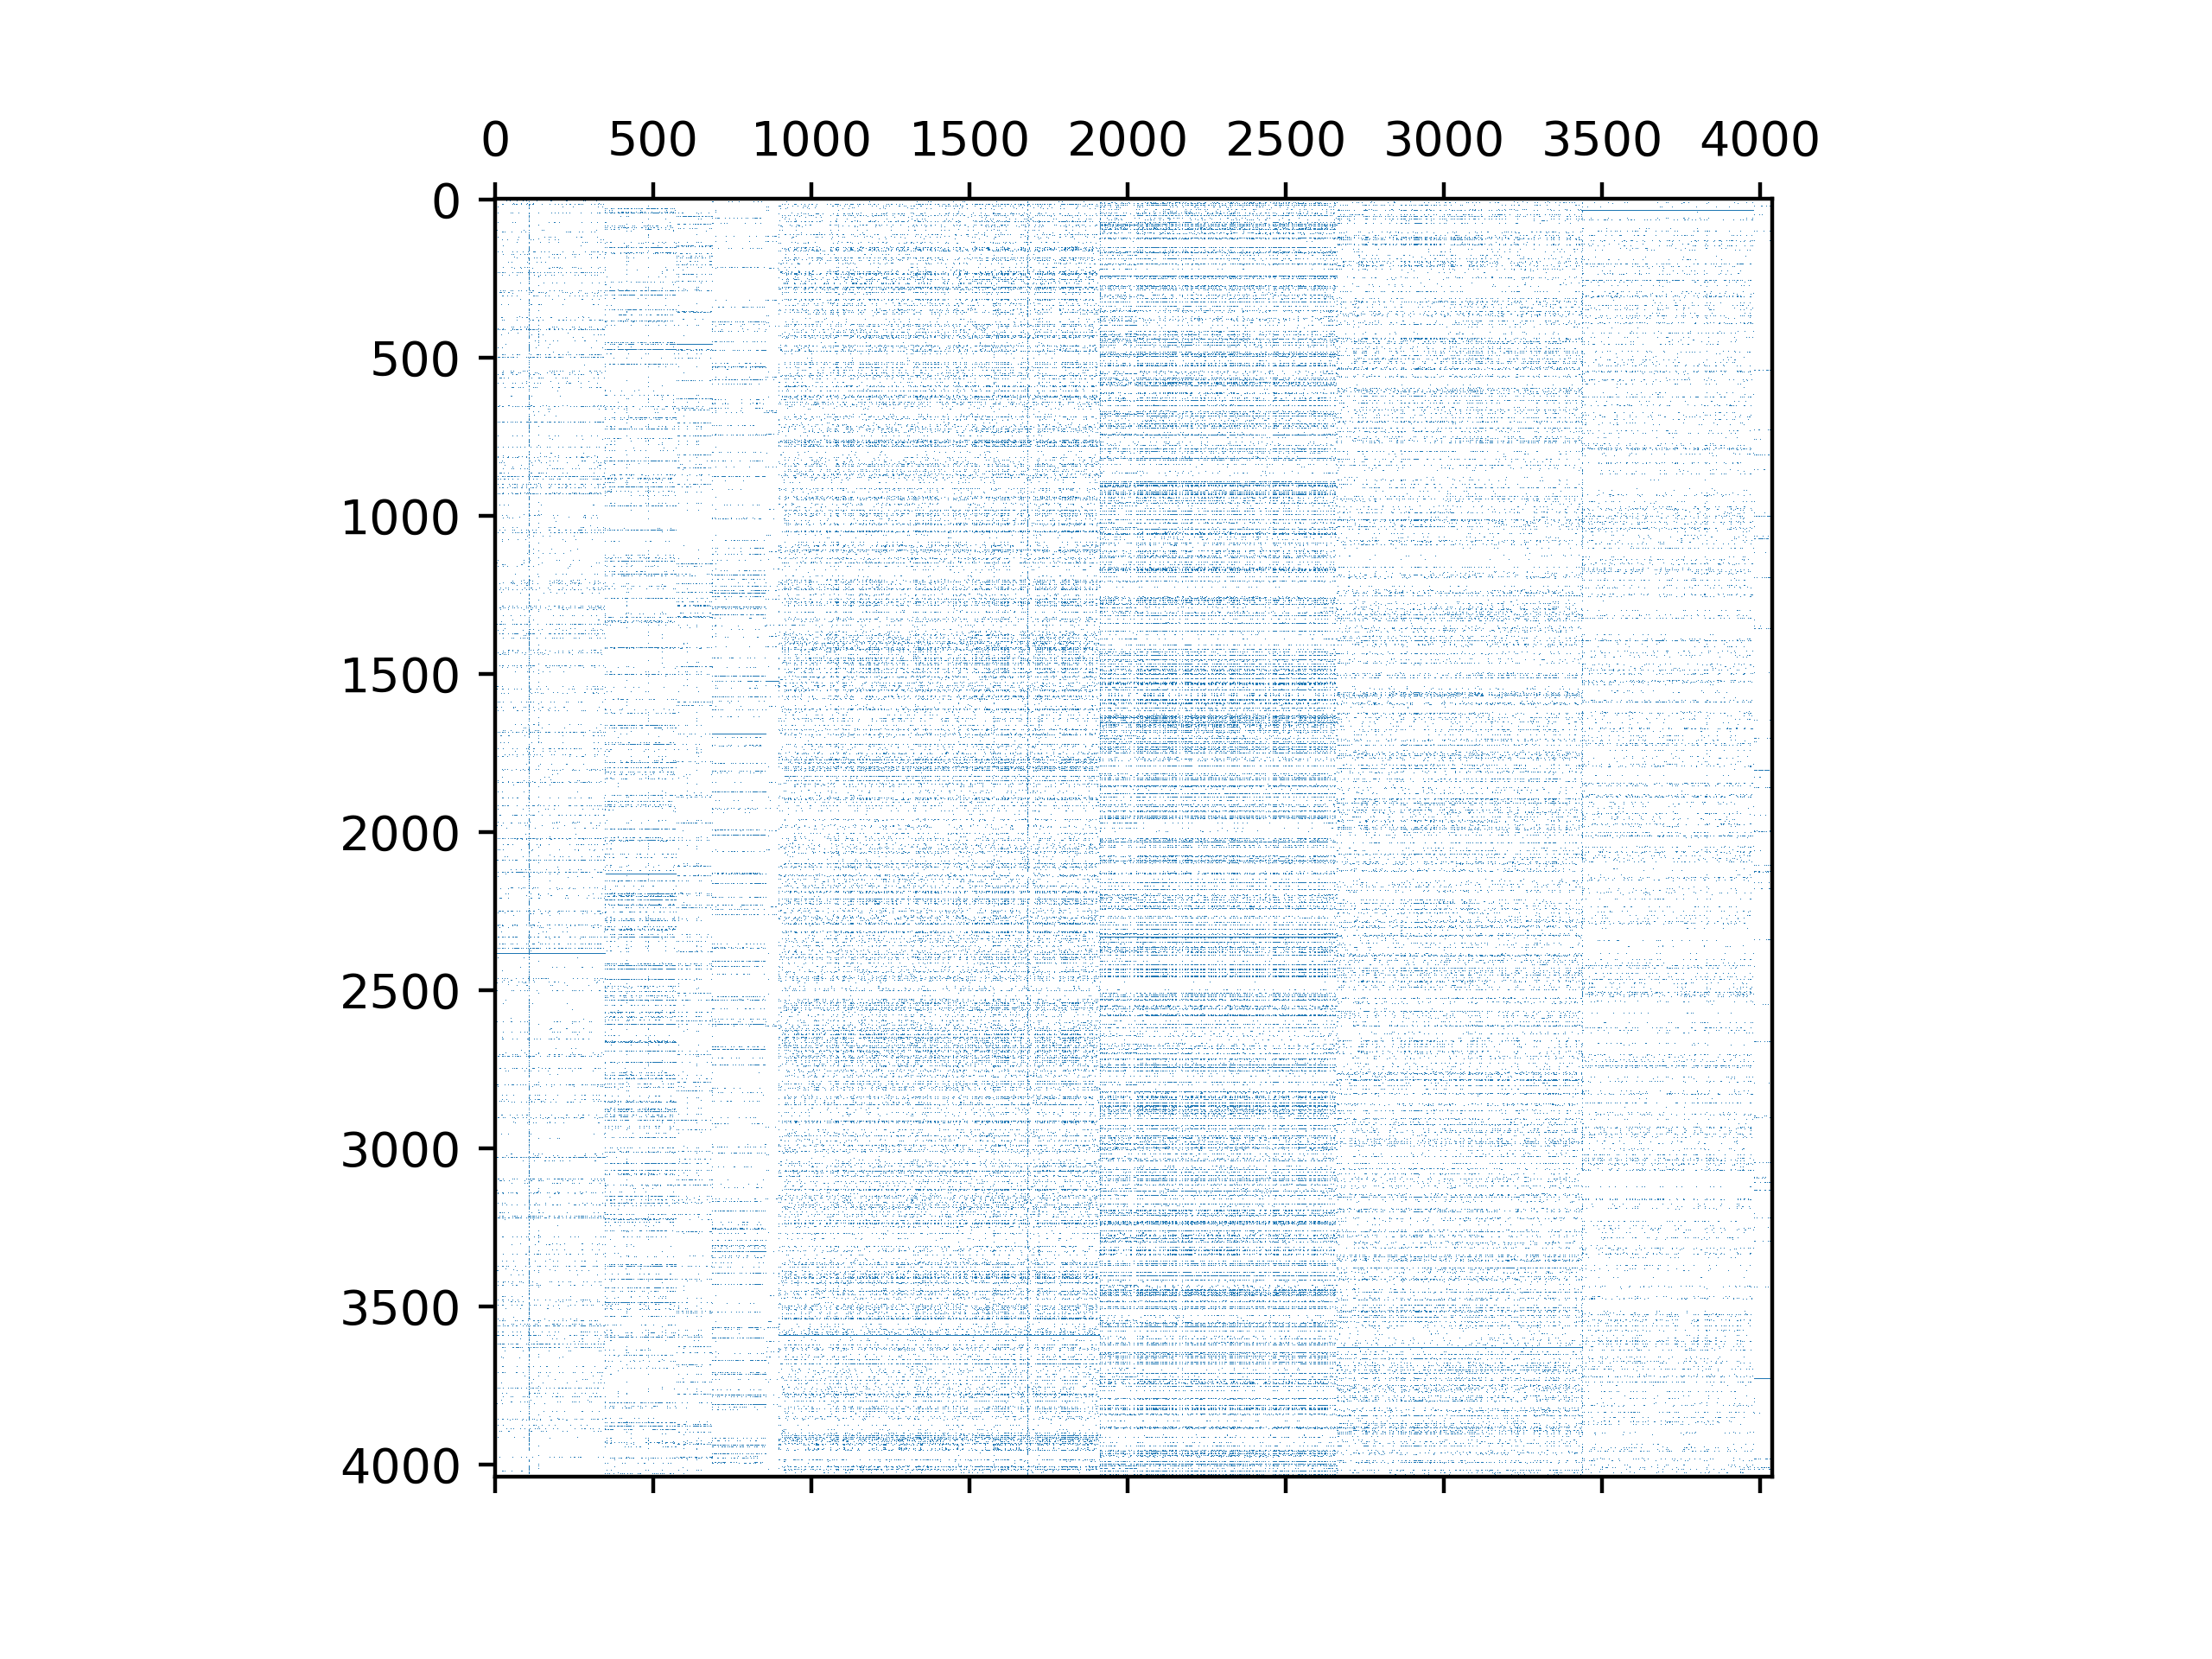
\includegraphics[width=5.5cm]{figures/fb-combined-rnd.png}}\hfil   
  \subfloat[Rabbit Order]{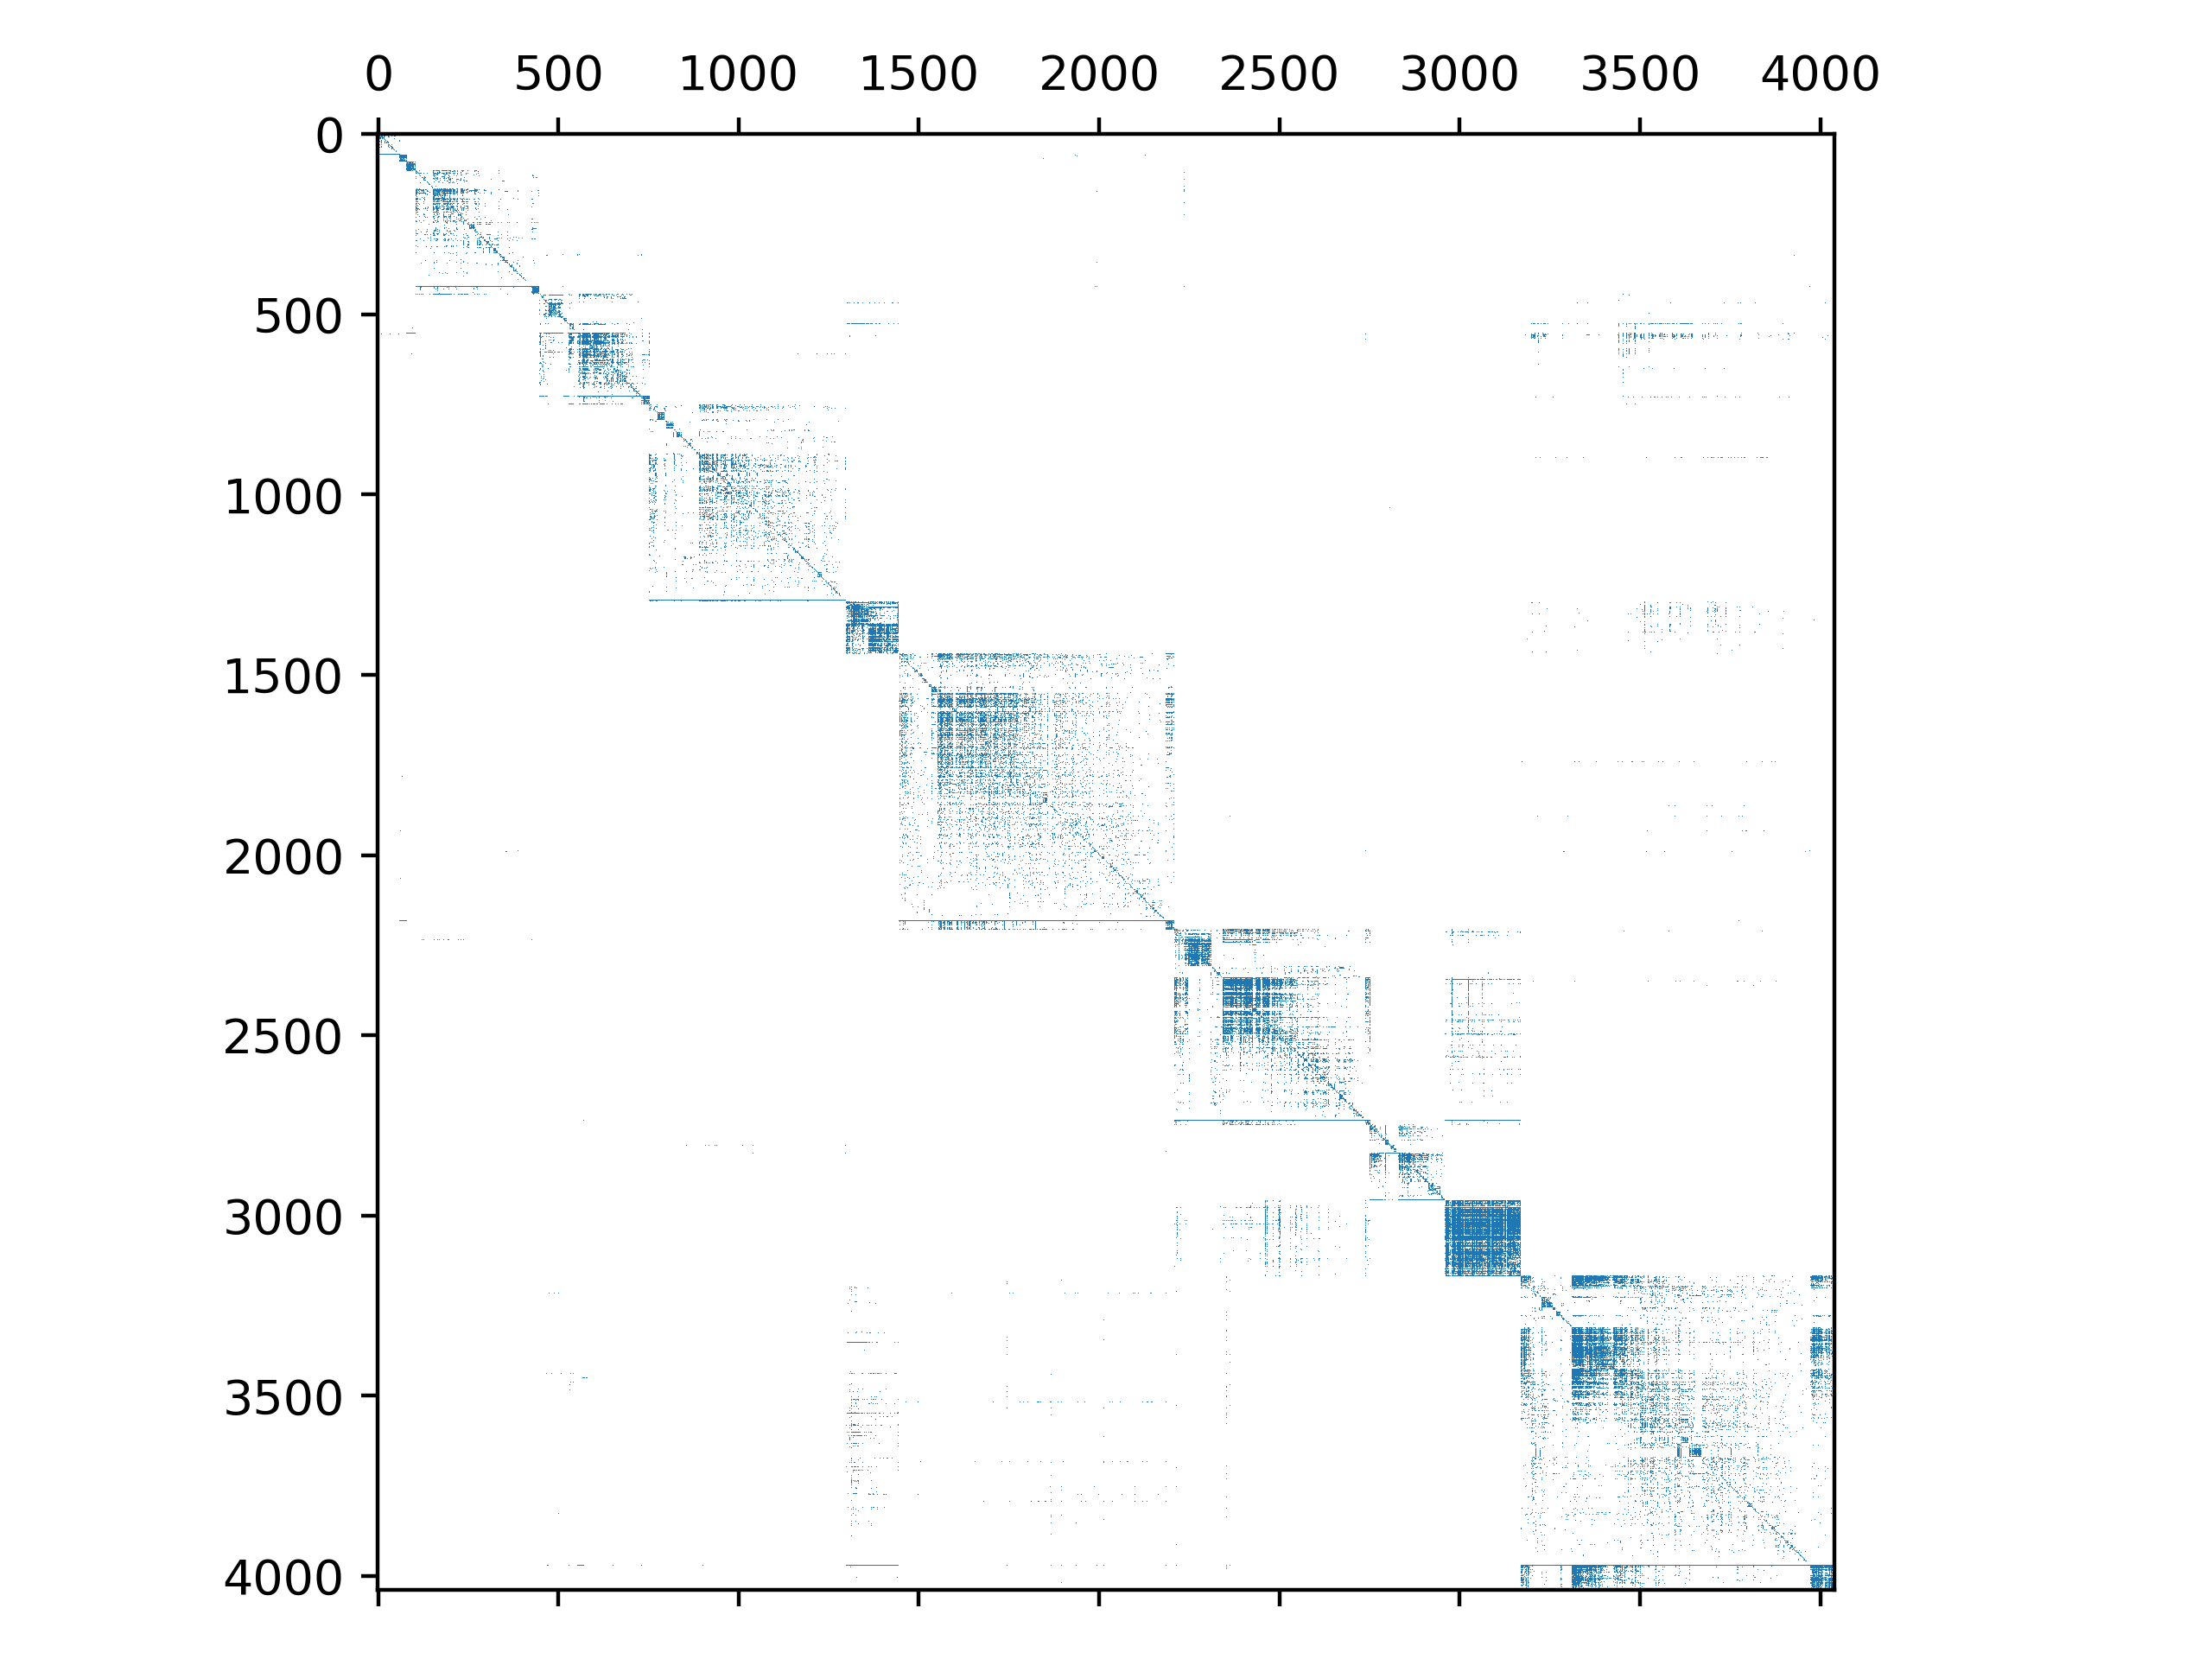
\includegraphics[width=5.5cm]{figures/fb-combined-rbt.png}}\hfil
  \subfloat[Cuthill-McKee Order]{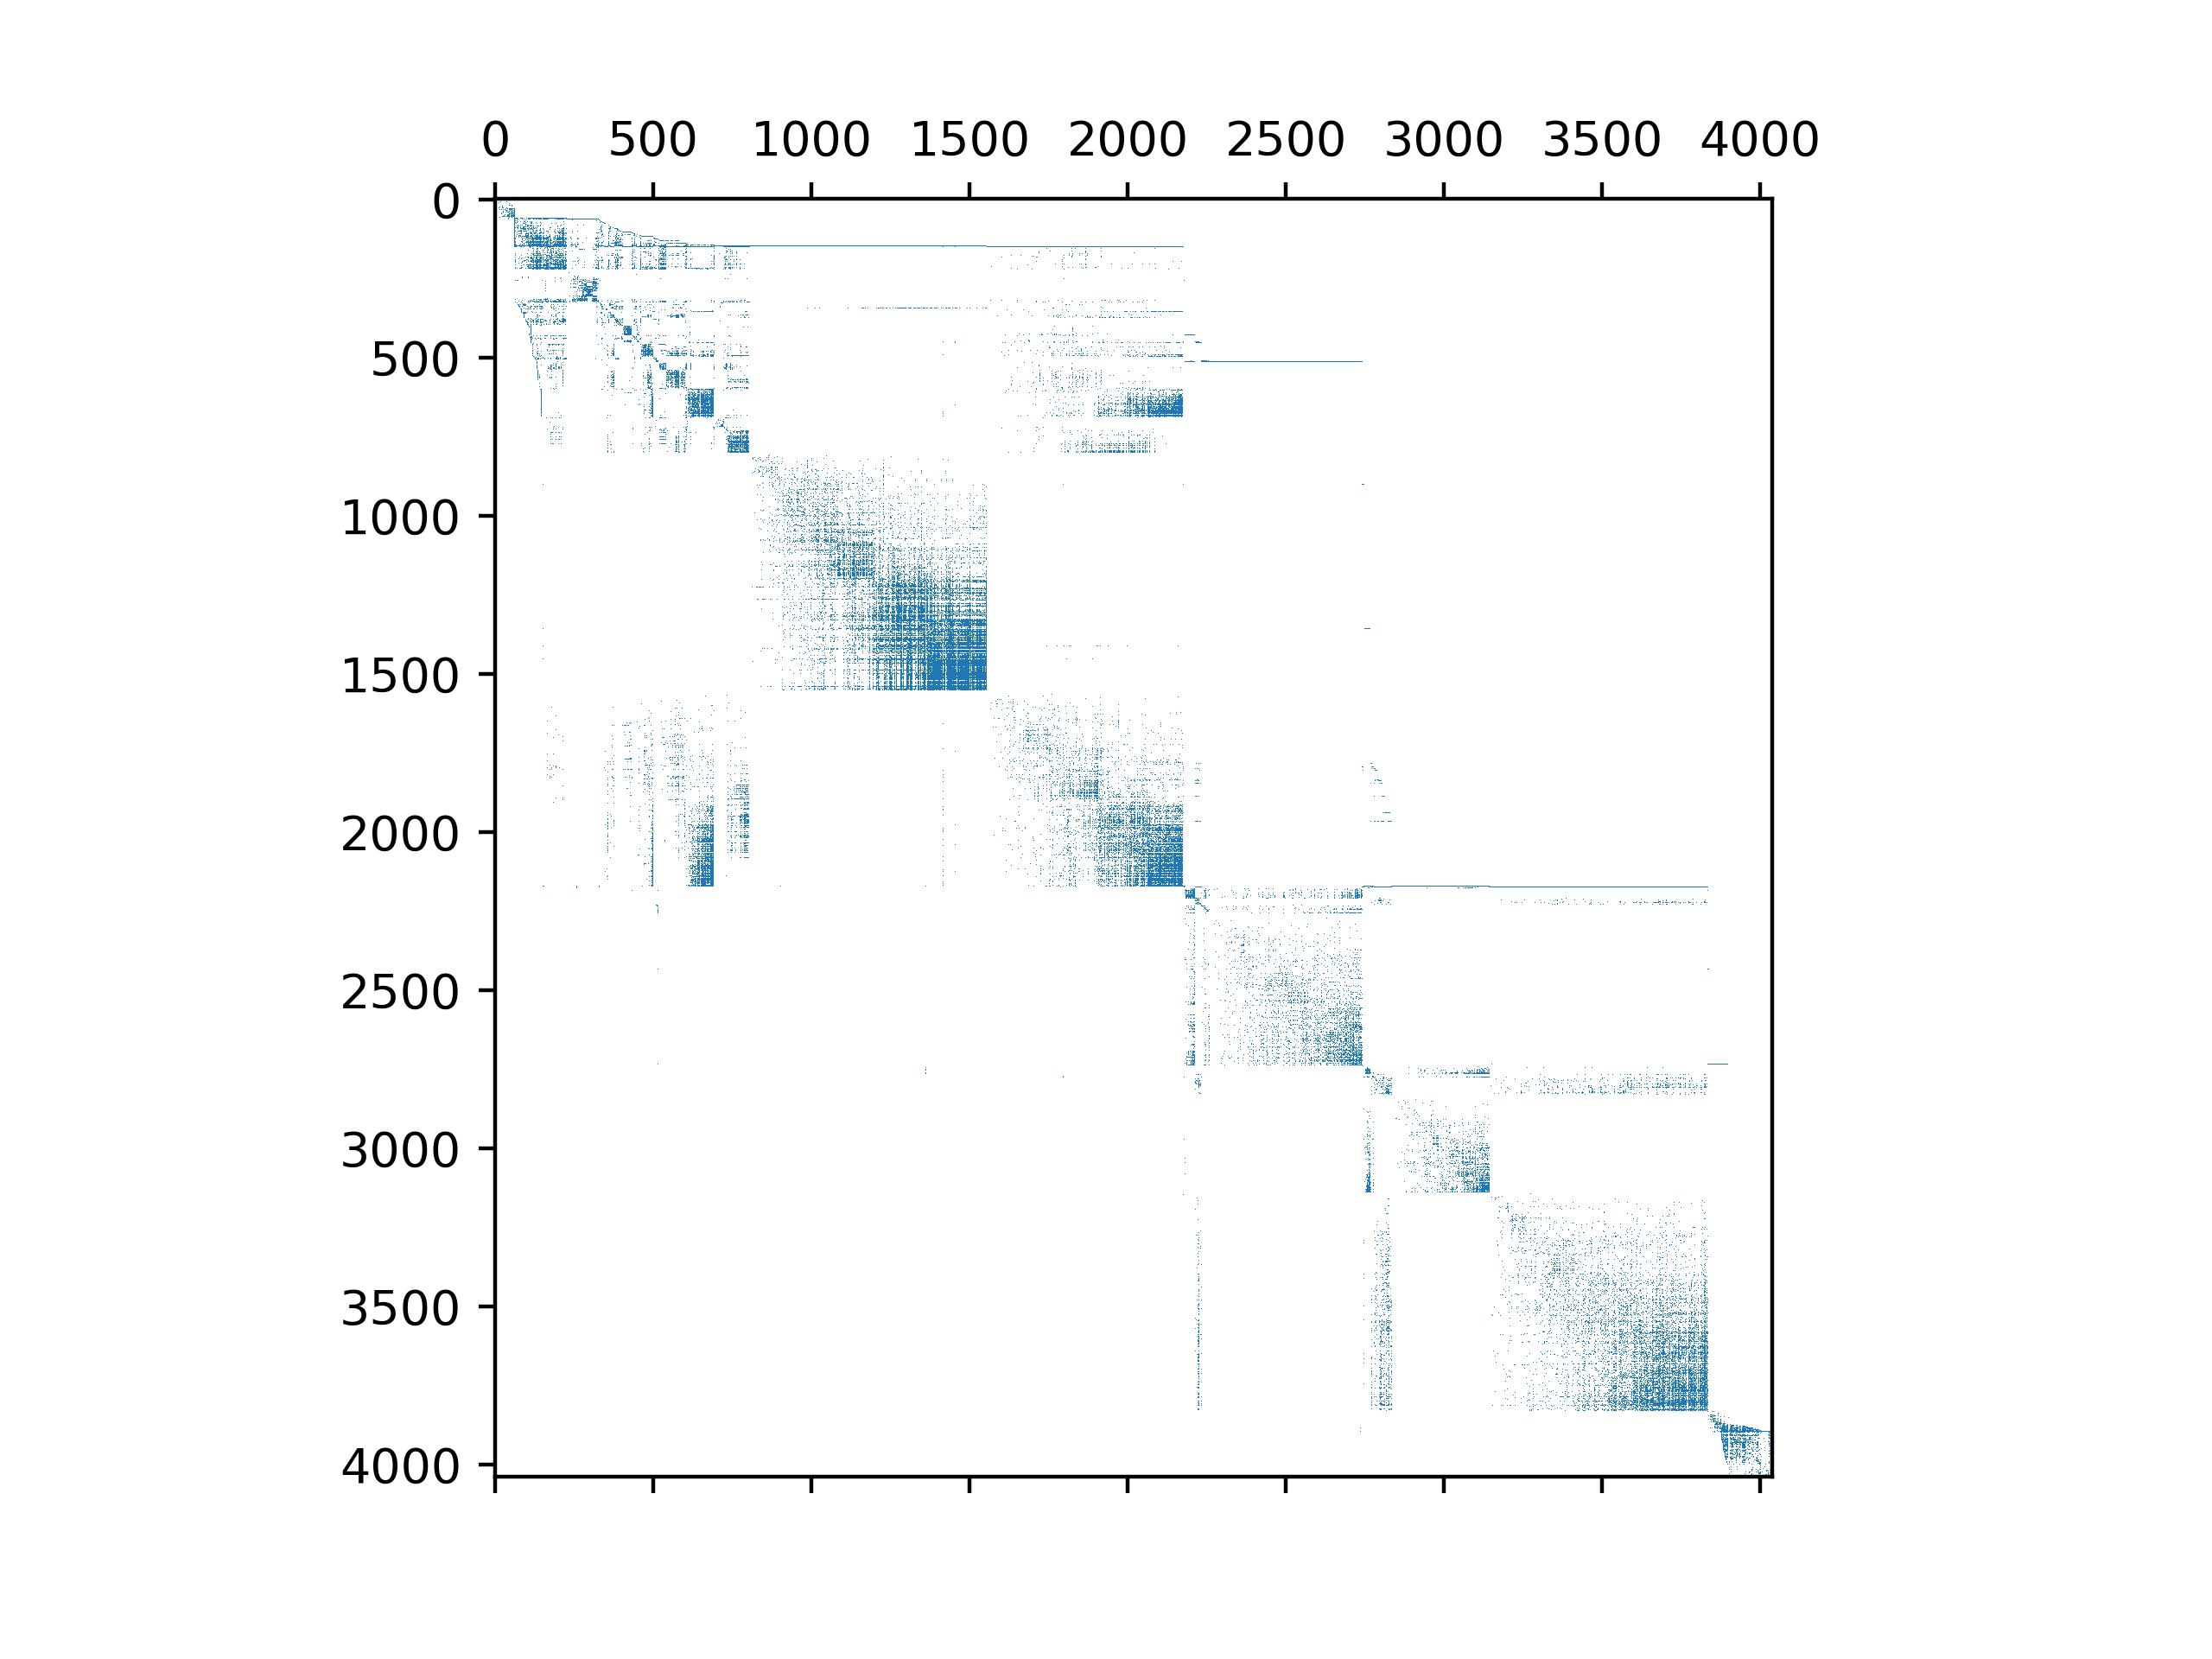
\includegraphics[width=5.5cm]{figures/fb-combined-rcm.png}}
  \caption{Adjacency matrices of an undirected Facebook Social Network graph with 4,039 vertices and 88,234 edges. Each pixel denotes an undirected edge (``friend-of'' relationship) between a pair of vertices (users) in the graph. Note the detected dense communities (submatrices) along the diagonal in (b) and the reduced bandwidth of the sparse matrix in (c). }\label{fig:fb_adjmats}
  \end{figure*}

To date, researchers have looked at \textit{either} vertex or edge ordering to optimize the performance of their \ac{VC} or \ac{EC} systems, but there has not been an extensive evaluation of possible \textit{vertex-and-edge} orderings. We define a \textbf{Vertex-and-Edge Ordering} of a graph as a preprocessing algorithm that:
\begin{enumerate}
    \item Reorders the \textit{vertices} to introduce structure into the adjacency matrix.
    \item Traverses the \textit{edges} using an edge ordering that leverages the structure of the isomorphic adjacency matrix. For example, the edge ordering could skip over large empty regions and traverse the dense regions using the \ac{HSFC}.
\end{enumerate}
This thesis is concerned in filling this knowledge gap and investigates the interaction between Vertex and Edge ordering. Namely, we answer the following research questions:

\textbf{RQ1}: It has been shown that vertex and edge ordering confer performance benefits in a variety of applications. Is it possible to combine vertex
and edge ordering as a preprocessing step such that the performance benefit gained by the combination of both is compounded (i.e., is greater than using either separately)?
\begin{itemize}
  \item Can edge-centric graph traversal be sped up by first introducing some structure into the adjacency matrix?
\end{itemize}

\textbf{RQ2}: Given an arbitrary input graph, is there a \textit{vertex-and-edge} ordering combination that yields the best performance for an \ac{EC} traversal (measured in speed of execution and number of cache misses)?

We answer these questions by making the following contributions. We:

\begin{enumerate}
  \item {Perform a preliminary performance evaluation on different vertex and edge orderings on single-threaded \ac{EC} traversals for a variety of graph datasets. We conclude that there \textit{does not} exist a one-size-fits-all \textit{vertex-and-edge} ordering that outperforms all others for all types of graphs.}
  \item {Derive an analytic model of performance using a dataset of graph features (statistical measures that summarize a graph) to identify the characteristics of a graph that help us determine which vertex-and-edge ordering performs best for \ac{EC} workloads.}
  \item {Develop a fully parallel implementation of the SlashBurn vertex ordering technique: \textbf{ParSB}.}
  \item {Propose a novel, lock-free, multithreaded vertex-and-edge ordering technique that leverages the compressed graph representation given by ParSB and traverses the edges of the graph using the \ac{HSFC}.}
  \item {Evaluate our novel vertex-and-edge ordering and compare its performance against locking-based and merging-based multithreaded vertex-and-edge orderings.}
\end{enumerate}

$<$here would be an outline of the thesis, detailing the sections of it, and what each section contains.$>$

\begin{enumerate}[label*=\arabic*.]
  \item {\textbf{Introduction}}
  \item {
    
    
  }
  \item {\textbf{Case Study: Does Vertex-and-Edge ordering affect performance?}
  To answer \textbf{RQ1}, we ran the following experiment on a dataset of $\approx 150$ graphs whose size ranges from modest ($\approx$30MB) to large ($\approx$40GB). For each graph, we computed 8 vertex orderings. For each vertex ordering, we completed 20 iterations of PageRank using either Row-major, Column-major, or the Hilbert Order. We saw that there was not a 1-size-fits-all vertex-and-edge ordering combination.
  Highlight the different results observed. Visualize dataset of graphs in (reduced) high-dimensional space (t-SNE, PCA) to try to identify clusters of graphs that behave similarly. Present a simple, interpretable model (decision tree, linear regression) that identifies the features that influence the performance of different vertex-and-edge orders.  
  }
  

  \item {\textbf{Parallel Slashburn}
  The results of the case study show that, for certain graphs, SlashBurn produced the greatest performance improvements. Motivated by this, we propose to parallelize this algorithm, to speedup the computation of this ordering 
  % (thereby producing a "somewhat-lightweight" vertex reordering.)
  Describe the SlashBurn algorithm in depth. Highlight subroutines of the algorithm that are parallelizable. Describe the Parallel Slashburn algorithm. Evaluate:
  \begin{itemize}
    \item The speedup between the sequential and parallel implementation.
    \item Scalability: speedup when increasing the number of threads.
    \item Equality of results: the orderings produced by the sequential and parallel implementations should be almost identical. 
    Show that this is the case by measuring the performance improvement that is gained by both implementations, and show how these improvements are practically identical.
  \end{itemize}
  }
  \begin{enumerate}[label*=\arabic*.]
    \item {\textbf{Modelling the \ac{WWR} of Real-world Graph}
    Define the \ac{WWR} of a graph: the number of iterations to compute the slashburn ordering $\times$ the number of hubs selected at each SlashBurn iteration.
    Note the differences in the \ac{WWR} among graphs. Observe that this metric is a deciding factor of whether to use the SlashBurn order or not. 
    Model the \ac{WWR} as a function of graph features. Use our model of \ac{WWR} to predict whether to iterate over the graph using our proposed HilBurn curve.
    }
  \end{enumerate}
  \item {\textbf{My Technique: Vertex-and-Edge Ordering using HilBurn}
    Given that we've seen combined speed ups using the combination of the SlashBurn Vertex Ordering and the Hilbert Edge Ordering, We propose the Hilbert+SlashBurn Vertex-and-Edge ordering, HilBurn.
    \begin{enumerate}
      \item First, reorder the vertices of the graph using the ordering produced by Parallel SlashBurn. 
      \begin{itemize}
      \item Use the analytic model that predicts the \ac{WWR} of a graph given its graph statistics to choose the number of hubs selected at each iteration. Use this model to optimize for a Wing Width that fits in the LLC.
      \item In the case where the \ac{WWR} is too large, we expect that HilBurn would not perform great, so use our model to pick an appropriate Vertex-and-Edge ordering based on the input graph's graph features. 
      \end{itemize}
      \item{
        Second, separate the reordered adjacency matrix into 4 ``zones'':
        \begin{enumerate}
          \item {
            \textbf{Upper Right Quadrant - URQ}: this region should fit in the LLC. This range is defined by: $[0, ki)$, where:
            \begin{itemize}
              \item  $k$ is the number of hubs selected at each Parallel Slashburn iteration
              \item  $i$ is the number of iterations it took to complete Parallel Slashburn
            \end{itemize}
            The URQ will be computed in parallel by splitting up the $ki \times ki$ quadrant of the adjacency matrix into subquadrants, each of which contains a copy of the vertex ids in the range of its subquadrant to ensure
            that no contention occurs while updating vertex data.
            At the end of each iteration, all threads merge the updates for the vertices in their subquadrants;
          }
          \item{\textbf{Right Wing}:
          Can be computed in parallel with URQ. The upper right wing will be split into quadrants based on the number of edges in each region - this is done to ensure a workload balance among the threads operating on the right wing.
          Each thread will own a non-overlapping region of the vertex id range: $[ki, N-1)$. No locks or merging required for this step.
          }
          \item{\textbf{Left Wing}:
          
          }
          \item{\textbf{Tail}}
        \end{enumerate}
      }
      
    \end{enumerate}
  }
  \item {\textbf{Evaluation}}
  \item {\textbf{Discussion}}
  \item {\textbf{Future Work}}
  \item \begin{enumerate}[label*=\arabic*.]
    \item {\textbf{SIMD Parallelism}}
    \item {\textbf{Further speedups using other state of the art (PQ, CCs, degree sorts)}}
  \end{enumerate}
  \item {\textbf{Conclusion}}

\end{enumerate}

% This document provides a quick set of instructions for using the
% \class{ubcdiss} class to write a dissertation in \LaTeX. 
% Unfortunately this document cannot provide an introduction to using
% \LaTeX.  The classic reference for learning \LaTeX\ is
% \citeauthor{lamport-1994-ladps}'s
% book~\cite{lamport-1994-ladps}.  There are also many freely-available
% tutorials online;
% \webref{http://www.andy-roberts.net/misc/latex/}{Andy Roberts' online
%     \LaTeX\ tutorials}
% seems to be excellent.
% The source code for this docment, however, is intended to serve as
% an example for creating a \LaTeX\ version of your dissertation.

% We start by discussing organizational issues, such as splitting
% your dissertation into multiple files, in
% \autoref{sec:SuggestedThesisOrganization}.
% We then cover the ease of managing cross-references in \LaTeX\ in
% \autoref{sec:CrossReferences}.
% We cover managing and using bibliographies with \BibTeX\ in
% \autoref{sec:BibTeX}. 
% We briefly describe typesetting attractive tables in
% \autoref{sec:TypesettingTables}.
% We briefly describe including external figures in
% \autoref{sec:Graphics}, and using special characters and symbols
% in \autoref{sec:SpecialSymbols}.
% As it is often useful to track different versions of your dissertation,
% we discuss revision control further in
% \autoref{sec:DissertationRevisionControl}. 
% We conclude with pointers to additional sources of information in
% \autoref{sec:Conclusions}.

% %%%%%%%%%%%%%%%%%%%%%%%%%%%%%%%%%%%%%%%%%%%%%%%%%%%%%%%%%%%%%%%%%%%%%%
% \section{Suggested Thesis Organization}
% \label{sec:SuggestedThesisOrganization}

% The \acs{UBC} \acf{GPS} specifies a particular arrangement of the
% components forming a thesis.\footnote{See
%     \url{http://www.grad.ubc.ca/current-students/dissertation-thesis-preparation/order-components}}
% This template reflects that arrangement.

% In terms of writing your thesis, the recommended best practice for
% organizing large documents in \LaTeX\ is to place each chapter in
% a separate file.  These chapters are then included from the main
% file through the use of \verb+\include{file}+.  A thesis might
% be described as six files such as \file{intro.tex},
% \file{relwork.tex}, \file{model.tex}, \file{eval.tex},
% \file{discuss.tex}, and \file{concl.tex}.

% We also encourage you to use macros for separating how something
% will be typeset (\eg bold, or italics) from the meaning of that
% something. 
% For example, if you look at \file{intro.tex}, you will see repeated
% uses of a macro \verb+\file{}+ to indicate file names.
% The \verb+\file{}+ macro is defined in the file \file{macros.tex}.
% The consistent use of \verb+\file{}+ throughout the text not only
% indicates that the argument to the macro represents a file (providing
% meaning or semantics), but also allows easily changing how
% file names are typeset simply by changing the definition of the
% \verb+\file{}+ macro.
% \file{macros.tex} contains other useful macros for properly typesetting
% things like the proper uses of the latinate \emph{exempli grati\={a}}
% and \emph{id est} (\ie \verb+\eg+ and \verb+\ie+), 
% web references with a footnoted \acs{URL} (\verb+\webref{url}{text}+),
% as well as definitions specific to this documentation
% (\verb+\latexpackage{}+).

% %%%%%%%%%%%%%%%%%%%%%%%%%%%%%%%%%%%%%%%%%%%%%%%%%%%%%%%%%%%%%%%%%%%%%%
% \section{Making Cross-References}
% \label{sec:CrossReferences}

% \LaTeX\ make managing cross-references easy, and the \latexpackage{hyperref}
% package's\ \verb+\autoref{}+ command\footnote{%
%     The \latexpackage{hyperref} package is included by default in this
%     template.}
% makes it easier still. 

% A thing to be cross-referenced, such as a section, figure, or equation,
% is \emph{labelled} using a unique, user-provided identifier, defined
% using the \verb+\label{}+ command.  
% The thing is referenced elsewhere using the \verb+\autoref{}+ command.
% For example, this section was defined using:
% \begin{lstlisting}
%     \section{Making Cross-References}
%     \label{sec:CrossReferences}
% \end{lstlisting}
% References to this section are made as follows:
% \begin{lstlisting}
%     We then cover the ease of managing cross-references in \LaTeX\
%     in \autoref{sec:CrossReferences}.
% \end{lstlisting}
% \verb+\autoref{}+ takes care of determining the \emph{type} of the 
% thing being referenced, so the example above is rendered as
% \begin{quote}
%     We then cover the ease of managing cross-references in \LaTeX\
%     in \autoref{sec:CrossReferences}.
% \end{quote}

% The label is any simple sequence of characters, numbers, digits,
% and some punctuation marks such as ``:'' and ``--''; there should
% be no spaces.  Try to use a consistent key format: this simplifies
% remembering how to make references.  This document uses a prefix
% to indicate the type of the thing being referenced, such as \texttt{sec}
% for sections, \texttt{fig} for figures, \texttt{tbl} for tables,
% and \texttt{eqn} for equations.

% For details on defining the text used to describe the type
% of \emph{thing}, search \file{diss.tex} and the \latexpackage{hyperref}
% documentation for \texttt{autorefname}.


% %%%%%%%%%%%%%%%%%%%%%%%%%%%%%%%%%%%%%%%%%%%%%%%%%%%%%%%%%%%%%%%%%%%%%%
% \section{Managing Bibliographies with \BibTeX}
% \label{sec:BibTeX}

% One of the primary benefits of using \LaTeX\ is its companion program,
% \BibTeX, for managing bibliographies and citations.  Managing
% bibliographies has three parts: (i) describing references,
% (ii)~citing references, and (iii)~formatting cited references.

% \subsection{Describing References}

% \BibTeX\ defines a standard format for recording details about a
% reference.  These references are recorded in a file with a
% \file{.bib} extension.  \BibTeX\ supports a broad range of
% references, such as books, articles, items in a conference proceedings,
% chapters, technical reports, manuals, dissertations, and unpublished
% manuscripts. 
% A reference may include attributes such as the authors,
% the title, the page numbers, the \ac{DOI}, or a \ac{URL}.  A reference
% can also be augmented with personal attributes, such as a rating,
% notes, or keywords.

% Each reference must be described by a unique \emph{key}.\footnote{%
%     Note that the citation keys are different from the reference
%     identifiers as described in \autoref{sec:CrossReferences}.}
% A key is a simple sequence of characters, numbers, digits, and some
% punctuation marks such as ``:'' and ``--''; there should be no spaces. 
% A consistent key format simiplifies remembering how to make references. 
% For example:
% \begin{quote}
%    \fbox{\emph{last-name}}\texttt{-}\fbox{\emph{year}}\texttt{-}\fbox{\emph{contracted-title}}
% \end{quote}
% where \emph{last-name} represents the last name for the first author,
% and \emph{contracted-title} is some meaningful contraction of the
% title.  Then \citeauthor{kiczales-1997-aop}'s seminal article on
% aspect-oriented programming~\cite{kiczales-1997-aop} (published in
% \citeyear{kiczales-1997-aop}) might be given the key
% \texttt{kiczales-1997-aop}.

% An example of a \BibTeX\ \file{.bib} file is included as
% \file{biblio.bib}.  A description of the format a \file{.bib}
% file is beyond the scope of this document.  We instead encourage
% you to use one of the several reference managers that support the
% \BibTeX\ format such as
% \webref{http://jabref.sourceforge.net}{JabRef} (multiple platforms) or
% \webref{http://bibdesk.sourceforge.net}{BibDesk} (MacOS\,X only). 
% These front ends are similar to reference managers such as
% EndNote or RefWorks.


% \subsection{Citing References}

% Having described some references, we then need to cite them.  We
% do this using a form of the \verb+\cite+ command.  For example:
% \begin{lstlisting}
%     \citet{kiczales-1997-aop} present examples of crosscutting 
%     from programs written in several languages.
% \end{lstlisting}
% When processed, the \verb+\citet+ will cause the paper's authors
% and a standardized reference to the paper to be inserted in the
% document, and will also include a formatted citation for the paper
% in the bibliography.  For example:
% \begin{quote}
%     \citet{kiczales-1997-aop} present examples of crosscutting 
%     from programs written in several languages.
% \end{quote}
% There are several forms of the \verb+\cite+ command (provided
% by the \latexpackage{natbib} package), as demonstrated in
% \autoref{tbl:natbib:cite}.
% Note that the form of the citation (numeric or author-year) depends
% on the bibliography style (described in the next section).
% The \verb+\citet+ variant is used when the author names form
% an object in the sentence, whereas the \verb+\citep+ variant
% is used for parenthetic references, more like an end-note.
% Use \verb+\nocite+ to include a citation in the bibliography
% but without an actual reference.
% \nocite{rowling-1997-hpps}
% \begin{table}
% \caption{Available \texttt{cite} variants; the exact citation style
%     depends on whether the bibliography style is numeric or author-year.}
% \label{tbl:natbib:cite}
% \centering
% \begin{tabular}{lp{3.25in}}\toprule
% Variant & Result \\
% \midrule
% % We cheat here to simulate the cite/citep/citet for APA-like styles
% \verb+\cite+ & Parenthetical citation (\eg ``\cite{kiczales-1997-aop}''
%     or ``(\citeauthor{kiczales-1997-aop} \citeyear{kiczales-1997-aop})'') \\
% \verb+\citet+ & Textual citation: includes author (\eg
%     ``\citet{kiczales-1997-aop}'' or
%     or ``\citeauthor{kiczales-1997-aop} (\citeyear{kiczales-1997-aop})'') \\
% \verb+\citet*+ & Textual citation with unabbreviated author list \\
% \verb+\citealt+ & Like \verb+\citet+ but without parentheses \\
% \verb+\citep+ & Parenthetical citation (\eg ``\cite{kiczales-1997-aop}''
%     or ``(\citeauthor{kiczales-1997-aop} \citeyear{kiczales-1997-aop})'') \\
% \verb+\citep*+ & Parenthetical citation with unabbreviated author list \\
% \verb+\citealp+ & Like \verb+\citep+ but without parentheses \\
% \verb+\citeauthor+ & Author only (\eg ``\citeauthor{kiczales-1997-aop}'') \\
% \verb+\citeauthor*+ & Unabbreviated authors list 
%     (\eg ``\citeauthor*{kiczales-1997-aop}'') \\
% \verb+\citeyear+ & Year of citation (\eg ``\citeyear{kiczales-1997-aop}'') \\
% \bottomrule
% \end{tabular}
% \end{table}

% \subsection{Formatting Cited References}

% \BibTeX\ separates the citing of a reference from how the cited
% reference is formatted for a bibliography, specified with the
% \verb+\bibliographystyle+ command. 
% There are many varieties, such as \texttt{plainnat}, \texttt{abbrvnat},
% \texttt{unsrtnat}, and \texttt{vancouver}.
% This document was formatted with \texttt{abbrvnat}.
% Look through your \TeX\ distribution for \file{.bst} files. 
% Note that use of some \file{.bst} files do not emit all the information
% necessary to properly use \verb+\citet{}+, \verb+\citep{}+,
% \verb+\citeyear{}+, and \verb+\citeauthor{}+.

% There are also packages available to place citations on a per-chapter
% basis (\latexpackage{bibunits}), as footnotes (\latexpackage{footbib}),
% and inline (\latexpackage{bibentry}).
% Those who wish to exert maximum control over their bibliography
% style should see the amazing \latexpackage{custom-bib} package.

% %%%%%%%%%%%%%%%%%%%%%%%%%%%%%%%%%%%%%%%%%%%%%%%%%%%%%%%%%%%%%%%%%%%%%%
% \section{Typesetting Tables}
% \label{sec:TypesettingTables}

% \citet{lamport-1994-ladps} made one grievous mistake
% in \LaTeX: his suggested manner for typesetting tables produces
% typographic abominations.  These suggestions have unfortunately
% been replicated in most \LaTeX\ tutorials.  These
% abominations are easily avoided simply by ignoring his examples
% illustrating the use of horizontal and vertical rules (specifically
% the use of \verb+\hline+ and \verb+|+) and using the
% \latexpackage{booktabs} package instead.

% The \latexpackage{booktabs} package helps produce tables in the form
% used by most professionally-edited journals through the use of
% three new types of dividing lines, or \emph{rules}.
% % There are times that you don't want to use \autoref{}
% Tables~\ref{tbl:natbib:cite} and~\ref{tbl:LaTeX:Symbols} are two
% examples of tables typeset with the \latexpackage{booktabs} package.
% The \latexpackage{booktabs} package provides three new commands
% for producing rules:
% \verb+\toprule+ for the rule to appear at the top of the table,
% \verb+\midrule+ for the middle rule following the table header,
% and \verb+\bottomrule+ for the bottom-most at the end of the table.
% These rules differ by their weight (thickness) and the spacing before
% and after.
% A table is typeset in the following manner:
% \begin{lstlisting}
%     \begin{table}
%     \caption{The caption for the table}
%     \label{tbl:label}
%     \centering
%     \begin{tabular}{cc}
%     \toprule
%     Header & Elements \\
%     \midrule
%     Row 1 & Row 1 \\
%     Row 2 & Row 2 \\
%     % ... and on and on ...
%     Row N & Row N \\
%     \bottomrule
%     \end{tabular}
%     \end{table}
% \end{lstlisting}
% See the \latexpackage{booktabs} documentation for advice in dealing with
% special cases, such as subheading rules, introducing extra space
% for divisions, and interior rules.

% %%%%%%%%%%%%%%%%%%%%%%%%%%%%%%%%%%%%%%%%%%%%%%%%%%%%%%%%%%%%%%%%%%%%%%
% \section{Figures, Graphics, and Special Characters}
% \label{sec:Graphics}

% Most \LaTeX\ beginners find figures to be one of the more challenging
% topics.  In \LaTeX, a figure is a \emph{floating element}, to be
% placed where it best fits.
% The user is not expected to concern him/herself with the placement
% of the figure.  The figure should instead be labelled, and where
% the figure is used, the text should use \verb+\autoref+ to reference
% the figure's label.
% \autoref{fig:latex-affirmation} is an example of a figure.
% \begin{figure}
%     \centering
%     % For the sake of this example, we'll just use text
%     %\includegraphics[width=3in]{file}
%     \Huge{\textsf{\LaTeX\ Rocks!}}
%     \caption{Proof of \LaTeX's amazing abilities}
%     \label{fig:latex-affirmation}   % label should change
% \end{figure}
% A figure is generally included as follows:
% \begin{lstlisting}
%     \begin{figure}
%     \centering
%     \includegraphics[width=3in]{file}
%     \caption{A useful caption}
%     \label{fig:fig-label}   % label should change
%     \end{figure}
% \end{lstlisting}
% There are three items of note:
% \begin{enumerate}
% \item External files are included using the \verb+\includegraphics+
%     command.  This command is defined by the \latexpackage{graphicx} package
%     and can often natively import graphics from a variety of formats.
%     The set of formats supported depends on your \TeX\ command processor.
%     Both \texttt{pdflatex} and \texttt{xelatex}, for example, can
%     import \textsc{gif}, \textsc{jpg}, and \textsc{pdf}.  The plain
%     version of \texttt{latex} only supports \textsc{eps} files.

% \item The \verb+\caption+ provides a caption to the figure. 
%     This caption is normally listed in the List of Figures; you
%     can provide an alternative caption for the LoF by providing
%     an optional argument to the \verb+\caption+ like so:
%     \begin{lstlisting}
%     \caption[nice shortened caption for LoF]{%
% 	longer detailed caption used for the figure}
%     \end{lstlisting}
%     \ac{GPS} generally prefers shortened single-line captions
%     in the LoF: multiple-line captions are a bit unwieldy.

% \item The \verb+\label+ command provides for associating a unique, user-defined,
%     and descriptive identifier to the figure.  The figure can be
%     can be referenced elsewhere in the text with this identifier
%     as described in \autoref{sec:CrossReferences}.
% \end{enumerate}
% See Keith Reckdahl’s excellent guide for more details,
% \webref{http://www.ctan.org/tex-archive/info/epslatex.pdf}{\emph{Using
% imported graphics in LaTeX2e}}.

% \section{Special Characters and Symbols}
% \label{sec:SpecialSymbols}

% \LaTeX\ appropriates many common symbols for its own purposes,
% with some used for commands (\eg \verb+\{}&%+) and
% mathematics (\eg \verb+$^_+), and others are automagically transformed
% into typographically-preferred forms (\eg \verb+-`'+) or to
% completely different forms (\eg \verb+<>+).
% \autoref{tbl:LaTeX:Symbols} presents a list of common symbols and
% their corresponding \LaTeX\ commands.  A much more comprehensive list 
% of symbols and accented characters is available at:
% \url{http://www.ctan.org/tex-archive/info/symbols/comprehensive/}
% \begin{table}
% \caption{Useful \LaTeX\ symbols}\label{tbl:LaTeX:Symbols}
% \centering\begin{tabular}{ccp{0.5cm}cc}\toprule
% \LaTeX & Result && \LaTeX & Result \\
% \midrule
%     \verb+\texttrademark+ & \texttrademark && \verb+\&+ & \& \\
%     \verb+\textcopyright+ & \textcopyright && \verb+\{ \}+ & \{ \} \\
%     \verb+\textregistered+ & \textregistered && \verb+\%+ & \% \\
%     \verb+\textsection+ & \textsection && \verb+\verb!~!+ & \verb!~! \\
%     \verb+\textdagger+ & \textdagger && \verb+\$+ & \$ \\
%     \verb+\textdaggerdbl+ & \textdaggerdbl && \verb+\^{}+ & \^{} \\
%     \verb+\textless+ & \textless && \verb+\_+ & \_ \\
%     \verb+\textgreater+ & \textgreater && \\
% \bottomrule
% \end{tabular}
% \end{table}

% %%%%%%%%%%%%%%%%%%%%%%%%%%%%%%%%%%%%%%%%%%%%%%%%%%%%%%%%%%%%%%%%%%%%%%
% \section{Changing Page Widths and Heights}

% The \class{ubcdiss} class is based on the standard \LaTeX\ \class{book}
% class~\cite{lamport-1994-ladps} that selects a line-width to carry
% approximately 66~characters per line.  This character density is
% claimed to have a pleasing appearance and also supports more rapid
% reading~\cite{bringhurst-2002-teots}.  I would recommend that you
% not change the line-widths!

% \subsection{The \texttt{geometry} Package}

% Some students are unfortunately saddled with misguided supervisors
% or committee members whom believe that documents should have the
% narrowest margins possible.  The \latexpackage{geometry} package is
% helpful in such cases.  Using this package is as simple as:
% \begin{lstlisting}
%     \usepackage[margin=1.25in,top=1.25in,bottom=1.25in]{geometry}
% \end{lstlisting}
% You should check the package's documentation for more complex uses.

% \subsection{Changing Page Layout Values By Hand}

% There are some miserable students with requirements for page layouts
% that vary throughout the document.  Unfortunately the
% \latexpackage{geometry} can only be specified once, in the document's
% preamble.  Such miserable students must set \LaTeX's layout parameters
% by hand:
% \begin{lstlisting}
%     \setlength{\topmargin}{-.75in}
%     \setlength{\headsep}{0.25in}
%     \setlength{\headheight}{15pt}
%     \setlength{\textheight}{9in}
%     \setlength{\footskip}{0.25in}
%     \setlength{\footheight}{15pt}

%     % The *sidemargin values are relative to 1in; so the following
%     % results in a 0.75 inch margin
%     \setlength{\oddsidemargin}{-0.25in}
%     \setlength{\evensidemargin}{-0.25in}
%     \setlength{\textwidth}{7in}       % 1.1in margins (8.5-2*0.75)
% \end{lstlisting}
% These settings necessarily require assuming a particular page height
% and width; in the above, the setting for \verb+\textwidth+ assumes
% a \textsc{US} Letter with an 8.5'' width.
% The \latexpackage{geometry} package simply uses the page height and
% other specified values to derive the other layout values.
% The
% \href{http://tug.ctan.org/tex-archive/macros/latex/required/tools/layout.pdf}{\texttt{layout}}
% package provides a
% handy \verb+\layout+ command to show the current page layout
% parameters. 


% \subsection{Making Temporary Changes to Page Layout}

% There are occasions where it becomes necessary to make temporary
% changes to the page width, such as to accomodate a larger formula. 
% The \latexmiscpackage{chngpage} package provides an \env{adjustwidth}
% environment that does just this.  For example:
% \begin{lstlisting}
%     % Expand left and right margins by 0.75in
%     \begin{adjustwidth}{-0.75in}{-0.75in}
%     % Must adjust the perceived column width for LaTeX to get with it.
%     \addtolength{\columnwidth}{1.5in}
%     \[ an extra long math formula \]
%     \end{adjustwidth}
% \end{lstlisting}


% %%%%%%%%%%%%%%%%%%%%%%%%%%%%%%%%%%%%%%%%%%%%%%%%%%%%%%%%%%%%%%%%%%%%%%
% \section{Keeping Track of Versions with Revision Control}
% \label{sec:DissertationRevisionControl}

% Software engineers have used \acf{RCS} to track changes to their
% software systems for decades.  These systems record the changes to
% the source code along with context as to why the change was required.
% These systems also support examining and reverting to particular
% revisions from their system's past.

% An \ac{RCS} can be used to keep track of changes to things other
% than source code, such as your dissertation.  For example, it can
% be useful to know exactly which revision of your dissertation was
% sent to a particular committee member.  Or to recover an accidentally
% deleted file, or a badly modified image.  With a revision control
% system, you can tag or annotate the revision of your dissertation
% that was sent to your committee, or when you incorporated changes
% from your supervisor.

% Unfortunately current revision control packages are not yet targetted
% to non-developers.  But the Subversion project's
% \webref{http://tortoisesvn.net/docs/release/TortoiseSVN_en/}{TortoiseSVN}
% has greatly simplified using the Subversion revision control system
% for Windows users.  You should consult your local geek.

% A simpler alternative strategy is to create a GoogleMail account
% and periodically mail yourself zipped copies of your dissertation.

% %%%%%%%%%%%%%%%%%%%%%%%%%%%%%%%%%%%%%%%%%%%%%%%%%%%%%%%%%%%%%%%%%%%%%%
% \section{Recommended Packages}

% The real strength to \LaTeX\ is found in the myriad of free add-on
% packages available for handling special formatting requirements.
% In this section we list some helpful packages.

% \subsection{Typesetting}

% \begin{description}
% \item[\latexpackage{enumitem}:]
%     Supports pausing and resuming enumerate environments.

% \item[\latexpackage{ulem}:]
%     Provides two new commands for striking out and crossing out text
%     (\verb+\sout{text}+ and \verb+\xout{text}+ respectively)
%     The package should likely
%     be used as follows:
%     \begin{verbatim}
%     \usepackage[normalem,normalbf]{ulem}
%     \end{verbatim}
%     to prevent the package from redefining the emphasis and bold fonts.

% \item[\latexpackage{chngpage}:]
%     Support changing the page widths on demand.

% \item[\latexpackage{mhchem}:] 
%     Support for typesetting chemical formulae and reaction equations.

% \end{description}

% Although not a package, the
% \webref{http://www.ctan.org/tex-archive/support/latexdiff/}{\texttt{latexdiff}}
% command is very useful for creating changebar'd versions of your
% dissertation.


% \subsection{Figures, Tables, and Document Extracts}

% \begin{description}
% \item[\latexpackage{pdfpages}:]
%     Insert pages from other PDF files.  Allows referencing the extracted
%     pages in the list of figures, adding labels to reference the page
%     from elsewhere, and add borders to the pages.

% \item[\latexpackage{subfig}:]
%     Provides for including subfigures within a figure, and includes
%     being able to separately reference the subfigures.  This is a
%     replacement for the older \texttt{subfigure} environment.

% \item[\latexpackage{rotating}:]
%     Provides two environments, sidewaystable and sidewaysfigure,
%     for typesetting tables and figures in landscape mode.  

% \item[\latexpackage{longtable}:]
%     Support for long tables that span multiple pages.

% \item[\latexpackage{tabularx}:]
%     Provides an enhanced tabular environment with auto-sizing columns.

% \item[\latexpackage{ragged2e}:]
%     Provides several new commands for setting ragged text (\eg forms
%     of centered or flushed text) that can be used in tabular
%     environments and that support hyphenation.

% \end{description}


% \subsection{Bibliography Related Packages}

% \begin{description}
% \item[\latexpackage{bibunits}:]
%     Support having per-chapter bibliographies.

% \item[\latexpackage{footbib}:]
%     Cause cited works to be rendered using footnotes.

% \item[\latexpackage{bibentry}:] 
%     Support placing the details of a cited work in-line.

% \item[\latexpackage{custom-bib}:]
%     Generate a custom style for your bibliography.

% \end{description}


% %%%%%%%%%%%%%%%%%%%%%%%%%%%%%%%%%%%%%%%%%%%%%%%%%%%%%%%%%%%%%%%%%%%%%%
% \section{Moving On}
% \label{sec:Conclusions}

% At this point, you should be ready to go.  Other handy web resources:
% \begin{itemize}
% \item \webref{http://www.ctan.org}{\ac{CTAN}} is \emph{the} comprehensive
%     archive site for all things related to \TeX\ and \LaTeX. 
%     Should you have some particular requirement, somebody else is
%     almost certainly to have had the same requirement before you,
%     and the solution will be found on \ac{CTAN}.  The links to
%     various packages in this document are all to \ac{CTAN}.

% \item An online
%     \webref{http://www.ctan.org/get/info/latex2e-help-texinfo/latex2e.html}{%
% 	reference to \LaTeX\ commands} provides a handy quick-reference
%     to the standard \LaTeX\ commands.

% \item The list of 
%     \webref{http://www.tex.ac.uk/cgi-bin/texfaq2html?label=interruptlist}{%
% 	Frequently Asked Questions about \TeX\ and \LaTeX}
%     can save you a huge amount of time in finding solutions to
%     common problems.

% \item The \webref{http://www.tug.org/tetex/tetex-texmfdist/doc/}{te\TeX\
%     documentation guide} features a very handy list of the most useful
%     packages for \LaTeX\ as found in \ac{CTAN}.

% \item The
% \webref{http://www.ctan.org/tex-archive/macros/latex/required/graphics/grfguide.pdf}{\texttt{color}}
%     package, part of the graphics bundle, provides handy commands
%     for changing text and background colours.  Simply changing
%     text to various levels of grey can have a very 
%     \textcolor{greytext}{dramatic effect}.


% \item If you're really keen, you might want to join the
%     \webref{http://www.tug.org}{\TeX\ Users Group}.

% \end{itemize}

\endinput

Any text after an \endinput is ignored.
You could put scraps here or things in progress.
